In this chapter, the methods to evaluate the impact of the techniques and technologies used by the case company on maintainabilty are explained. This study follows the triangulation strategy \cite{51}. This strategy is applied by conducting two different methods within the scope of this study. These methods are quantitative and qualitative evaluations. Quantitative evaluation is made using object-oriented software maintainability metrics, and qualitative evaluation was made via interviews and surveys with Android developers. In this way collecting data from different resources is ensured, and more coherent results can be obtained. Another reason for using this method is that the study subject is closely related to the industry. Due to this close relationship, it is predicted that qualitative evaluations of the Android community and Android developers could increase the accuracy of this study. Thus, maximum efficiency by going beyond the traditional quantitative measurement techniques is aimed. Also, why and how these methods are chosen are explained in this chapter. Hence, the first research question is answered.

\subsection{Qualitative Evaluation}
When other academic studies dealing with the measurement of maintainability of software systems were reviewed, it was seen that many studies use quantitative methods. When the quantitative evaluations made in these studies are examined, it is seen that Android applications use several object-oriented software metrics while evaluating maintainability. Details of these studies were shared earlier in section \ref{section:3.2}. Although it cannot be claimed that such quantitative measurements are inaccurate, it would not be wrong to say that these measures are inadequate at times. It is essential to make qualitative evaluations and quantitative evaluations to increase the efficiency of the evaluations. In this way, it may be possible to measure developers' experiences and their effects on maintainability. For these reasons, an Android developer survey and interviews were conducted within this study's scope. This section covers these qualitative methods.

\subsubsection{Android Developer Survey}
\label{section:4.1.1}
The survey accepted answers between April 2020 and March 2021 and reached 164 participants in total.
\begin{figure}[ht!]
    \centering
    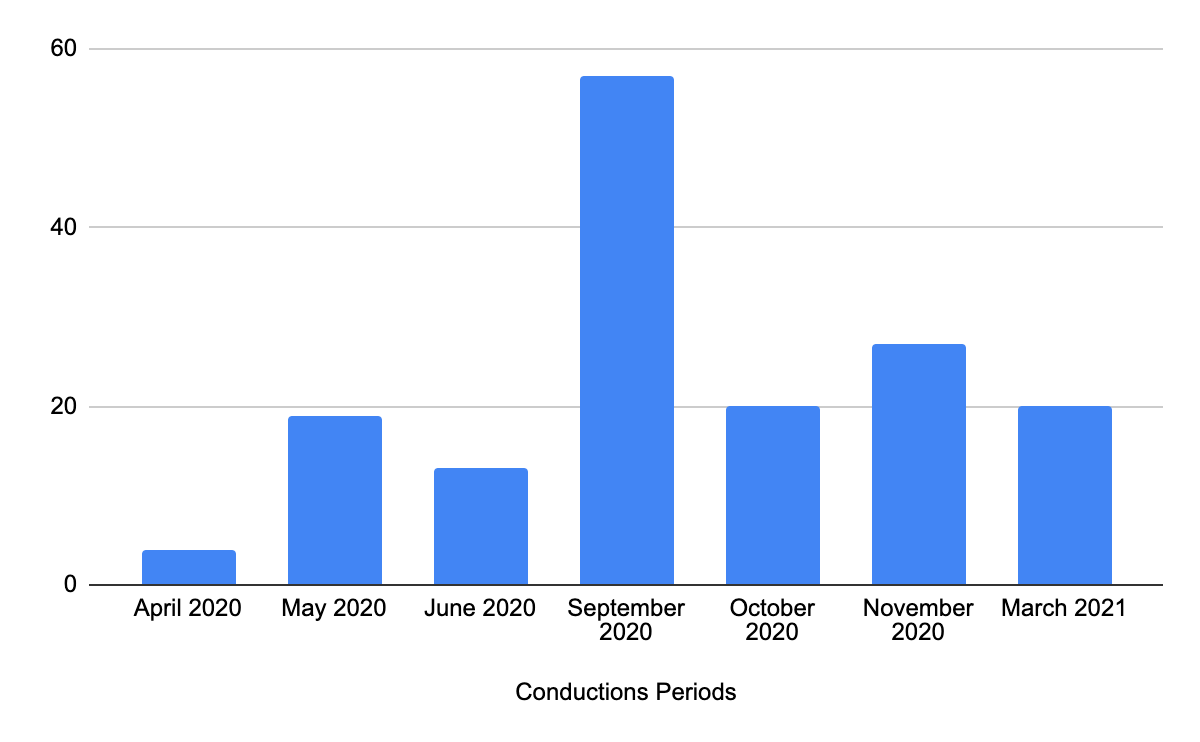
\includegraphics[scale=0.3]{figures/survey_conduction_period.png}
    \caption{Conduction period results}
    \label{fig:conduction_period}
\end{figure}

As shown in Fig. \ref{fig:conduction_period}, participation in the survey took place only during specific periods of this one-year term. Although the questionnaire accepted answers for a year-long, it was boosted in different periods,  as shown in the histogram above. It would be logical to consider this situation while examining the response numbers.

\subsubsection{Interviews with Team Members}
\label{section:4.1.2}
The second step of the qualitative evaluations carried out within this study’s scope is the interviews conducted with Mooncascade's Android team members.  The interview questions are designed to qualitatively evaluate the techniques and technologies used by Mooncascade's Android team in terms of maintainability. Also, the interviews aim to determine the importance of maintainability from the case company's point of view.  Thus, proving or disproving the study's claim that maintainability is a key concept to overcome the issues mentioned in the problem statement section would be possible. Eight questions were determined for these purposes. Below are listed the questions asked to each member of Mooncascade's Android team during these interviews:
\begin{itemize}
    \item How many years of experience do you have as an Android developer? Please specify the years in Mooncascade and other companies.
    \item How many different Android projects have you completed in Mooncascade, and how many different domains did those projects belong to?
    \item What is your understanding of maintainability in the context of software engineering?
    \item As an employee of a software development company that provides services to the different domains, what makes maintainability more essential for you?
    \item What is the importance of maintainability when developing Android applications?
    \item What is the most critical aspect for maintainability when developing Android applications (e.g. architecture, libraries, programming language, etc.)?
    \item How do you think the current technology stack of the team impacts Android applications’ maintainability? Please specify for each item below:
    \begin{itemize}
        \item Programming Languages(Kotlin/Java)
        \item Software Engineering principles (SOLID/Clean Code)
        \item Architecture (MVVM/Clean)
        \item Libraries (RxJava, Dagger 2, Apollo/Retrofit)
        \item Android Architecture Components (ViewModel, LiveData, Room, etc.)
    \end{itemize}
    \item What could be improved in our current tech stack and the principles we apply to improve the Android applications’ maintainability?
\end{itemize}

Three main criteria were taken into consideration while preparing these questions. First of all, questions were chosen to get to know about the participants' background and experience. Later, some questions were designed to learn participants' understanding of maintainability in software engineering. Lastly, questions were drafted to learn about participants' thoughts about the impact of technologies and principles used by Mooncascade on maintainability. The interview was conducted privately with each team member.  It is aimed that the data gathered through these interviews will increase the accuracy and validity of evaluations.


\subsection{Maintainability Evaluation with Object-Oriented Metrics}
\label{section:4.2}
In this section, the results obtained from the interviews made with the members of the Mooncascde Android team within the scope of qualitative measurements are shared.

\subsubsection{Conduction}
The questions mentioned in the interview, the details of which are shared in section \ref{section:3.1.2}, were conducted with the members of Mooncascade's Android team within the scope of qualitative evaluations. Interviews were conducted online, privately with each member of the team. The team was eight in total, and every team member, except the author of this study, participated in these interviews. The interviews took place in April 2021, and all the responses of the team members were kept in written and video record format. Subsequently, the presentation of the results was realized as a result of the rewording of these records.

\subsubsection{Participant Background}
The first three questions of the interview were designed to understand the competencies of the participants in the field of Android application development and to see how well their knowledge are regarding the concept of maintainability in software engineering. When the answers given to these questions were examined, it was seen that the participants had an Android application development experience ranging from 3 to 10 years. In addition, the participants stated that they accomplished many Android projects in different fields, and the Android applications implemented through these projects are the applications that are actively used today. Considering the knowledge levels of the participants about maintainability in software systems, it was seen that the participants emphasized the areas of readability, understandability, modifiability and up-to-dateness. Without exception, all the participants highlighted these concepts in their answers to the questions related to the understanding of software maintainability.

\subsubsection{Importance of the Maintainability}
The fourth, fifth and sixth questions of the interviews are designed to determine the importance of maintainability for the case company.

The fourth question of the interview asked the participants the importance of maintainability for the case company. Five of the participants stated that maintainability is an essential requirement for the company due to how the company works. Since the company works for different customers from different fields and the developer circulation in these projects is high, these participants stated that the maintainability of the projects is critical in terms of cost, time and effort. These participants emphasized that it is vital for the company to develop Android applications with high understandability, high modifiability, and high maintainability due to facilitating the development, hand over of the projects to the customer and maintenance operations required in the long term. Also, two participants stated that maintainability is already critical for software systems and that there is no extra situation that makes it more important for the company.

The fifth question of the interview asked the participants the importance of maintainability for the Android applications. Four of the participants stated that maintainability is important in solving the complexity issues in Android applications. Also, the participants stated that the fact that the Android platform and third-party Android libraries are evolving rapidly makes the maintainability of the Android application crucial. Participants stated  that if unstable libraries are preferred for the sake of the industry trends the fast evolution of the platform may cause problems in terms of maintainability. Also, two participants stated that maintainability is already important for software systems and that there is no extra situation that makes it more important for the Android applications.

The sixth question of the interview asked the participants for the most important matter for Android applications when it comes to maintainability. In general, it was seen that the participants provided 2 different answers to this question rather than stating a single matter. When the responses of the participants are examined, it is seen that the application architecture is emphasized four times, the third-party libraries emphasized 4 times, and the documentation once. The reason why third-party libraries affect maintainability was explained in the previous paragraph. It was seen that the developers put the same emphasis when answering this question as well. In addition, it was emphasized by the participants that the choice of architecture increases the maintainability of the applications as it makes the codebases of the applications better structured, standardized and consistent. Lastly, one participant stated that the documenting of the Android codebases improves understandability.

\subsubsection{Qualitative Evaluations}
The last two interview questions were directed to the participants to qualitatively evaluate the methods and technologies used by the company while developing Android applications  (see section \ref{section:2.3}) from the maintainability point  of view. 

When the responses of the participants are examined, positive comments about Kotlin programming language draw attention. Kotlin was found to be more concise and more readable than Java by the participants, and the participants stated that this situation has a positive effect on maintainability. Also, one participant stated that programming language did not have any positive or negative effect on maintainability. 

When looking at the answers about the SOLID and Clean Code principles, again, mostly positive reviews are seen. Participants think that the impact of these principles are positive on maintainability in terms of regulating the coding conventions of their codebases, increasing readability, facilitating separation of concerns and increasing consistency. 

On the subjects of architecture and design patterns, the participants stated that they found the MVVM design pattern positive for maintainability for it decreasing the coupling level between the classes responsible for view and presentation. Besides, the support of the Android Architecture Components framework offered by Google's Android team for MVVM and the fact that this framework was seen as a stable framework by the participants were considered positively by the participants in terms of maintainability. In the case of Clean Architecture, most participants stated that this architecture successfully managed to separate concerns, thus reducing the complexity and coupling levels of Android codebases, therefore increase the maintainability of the Android applications. However, these participants also stated that this architecture increases the complexity of small and medium-sized projects and decreases the readability of the codebase thus negatively impact the maintainability. 

It was observed that the participants made different comments about the effect of the third-party libraries used by the team on the maintainability of the applications. For example, the RxJava library was criticized in different ways. Participants stated that the steep learning curve of the RxJava library decreases the understandability of Android applications. Thus maintainability was negatively affected. In addition, the risk of RxJava becoming obsolete in the near future was also stated by some participants. It was mentioned that this situation had a negative effect on maintainability. On the other hand, some participants stated that this library has positive effects on maintainability due to its strong community, documentation and advanced features. Participants stated that Dagger 2 library has a positive impact on maintainability since it is a reliable and well-documented library supported by the Google Android team as a standard way of dependency injection. On the other hand, it was emphasized by the two participants that the complex structure of this library and its steep learning curve may cause problems in readability and understandability and that maintainability may be negatively affected. Regarding the Retrofit and Apollo libraries, all of the participants stated that these libraries have positive effects on maintainability. Reasons for that mentioned by the participants as strong community support and documentation, stability and reliability. In addition, the participants stated that the Retrofit library had become the industry standard, and it has a positive effect in terms of maintainability as it is easier to use than other alternatives. Architecture Components framework offered by Google's Android team has also found handy by the participants when it comes to the maintainability of Android applications. And as stated before, the reason for that is that the framework was seen as a stable framework by the participants and considered positively by the participants in terms of maintainability. However, one participant has stated that due to some internal issues that this framework has, the framework might badly affect maintainability. 

Ultimately, participants also stated that improvements can be made in the currently used methods and technologies. It is seen that the participants mentioned that the documentation of the Android applications could be improved. Also, they also mentioned that libraries can be reconsidered based on the current trends and up to date technologies.
